\label{Section:approach}
Before going into the experiment details, we has evaluated the relationship among AMR refinement resolution, CPU power level and the energy consumption. As shown in the Figure \ref{fig:Energy_consumption_trend}, the execution time will increase as the level of refinement/resolution increases or cap down CPU power. The energy consumption presents the same trend as the execution time, i.e., LMC will consume more energy as the levels of refinement/resolution increase or capping down CPU power. The question here is how to use this characterization to create available power budget. We propose to combine these two factors, adjusting resolution and applying appropriate power capping, to get available power budget for running other tasks (e.g., checkpointing). 


\textbf{Configuration}
\begin{table}[H]
\begin{center}
\begin{tabular}{|l|l|}
	\hline
	\textbf{Parameter} & \textbf{Value}\\ \hline
    Platform & CAPER cluster\\ 		\hline
    Number of cores & 64 cores\\
	\hline
	Resolution & level 3 2 1\\
    \hline
    Time step & 10\\
    \hline
    Time unit & Second\\
    \hline
    Power measurement & RAPL meter\\
    \hline
    Power cap & RAPL\\
    \hline
\end{tabular}
\end{center}
\caption{Configuration for experiment of getting available power budget through power capping and resolution degradation
}
\label{table:table_tradeoff}
\end{table}



\begin{figure}[H]
	\centering
    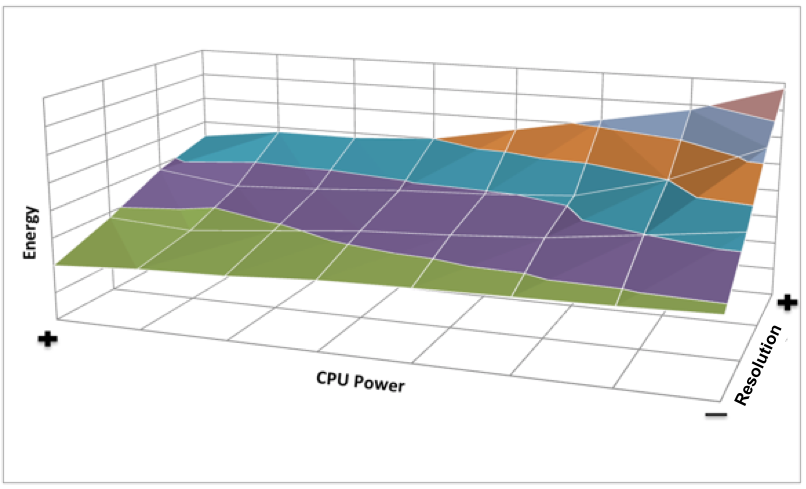
\includegraphics[width=8cm]{figs/Energy_consumption_trend.png}
        \caption{Energy consumption trend for different power caps and refinement levels}
        \label{fig:Energy_consumption_trend}
\end{figure}

\begin{figure}[H]
	\centering
    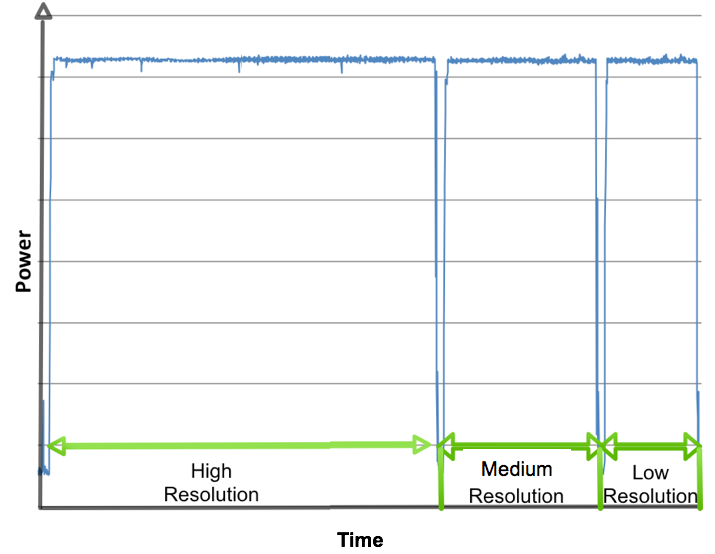
\includegraphics[width=8cm]{figs/LMCruntime.png}
        \caption{LMC power consumption curve with different (qualitative) resolution levels on 64 cores}
        \label{fig:LMCruntime}
\end{figure}


\begin{figure}[H]
	\centering
    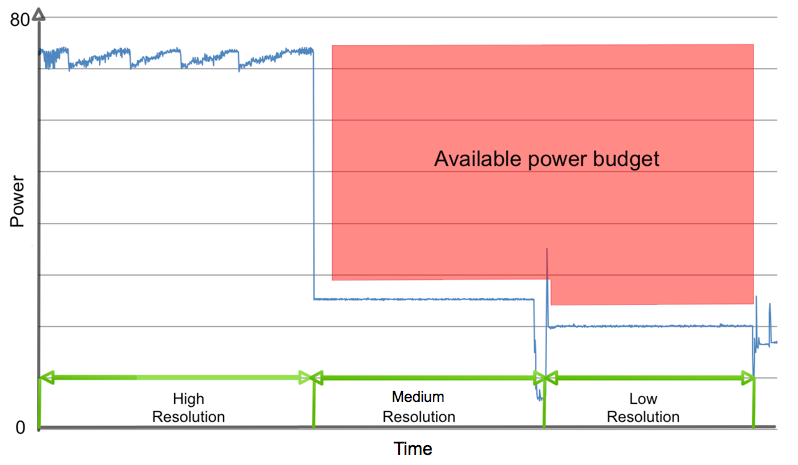
\includegraphics[width=8cm]{figs/Available_power_budget.png}
        \caption{Available power budget from applying resolution degradation and appropriate power capping}
        \label{fig:Available_power_budget}
\end{figure}


To briefly demonstrate this concept, we measure the LMC execution time with different resolution levels on 64 cores, as shown in Figure \ref{fig:LMCruntime}. Obviously, the execution time is decreasing as we degrading the resolution levels. In the meantime, capping down the CPU power will increase the execution time. Therefore, if applying appropriate power capping to it, then each execution can be the same. In the work, since we define the execution time as the performance criteria, by adjusting resolution and applying appropriate power capping, we can keep the performance while having the available power budget, shown as the red shadow area in Figure \ref{fig:Available_power_budget}.



